\input{mmd-beamer-header}
\def\mytitle{MultiMarkdown Support for Beamer}
\def\subtitle{A quick example}
\def\myauthor{Fletcher T. Penney}
\def\affiliation{http:/\slash fletcherpenney.net\slash }
\def\copyright{2009-2011 Fletcher T. Penney.  \\
This work is licensed under a Creative Commons License.  \\
http:/\slash creativecommons.org\slash licenses\slash by-sa\slash 2.5\slash }
\def\latexmode{beamer}
\def\latexxslt{beamer}
\def\event{MMD Beamer Announcement}
\def\mydate{August 13, 2009}
\def\theme{keynote-gradient}
\input{mmd-beamer-begin-doc}
\part{MultiMarkdown and Beamer}
\label{multimarkdownandbeamer}

\section{What is it?}
\label{whatisit}

\begin{frame}

\frametitle{What is MultiMarkdown?}
\label{whatismultimarkdown}

\href{http://fletcherpenney.net/multimarkdown/}{MultiMarkdown}\footnote{\href{http://fletcherpenney.net/multimarkdown/}{http:/\slash fletcherpenney.net\slash multimarkdown\slash }} is a derivative of John Gruber's \href{http://daringfireball.net/projects/markdown/}{Markdown}\footnote{\href{http://daringfireball.net/projects/markdown/}{http:/\slash daringfireball.net\slash projects\slash markdown\slash }}.

Basically, it converts plain text into pretty documents:

\begin{itemize}
\item HTML

\item PDF

\item RTF

\item and, now, PDF presentations

\end{itemize}

\end{frame}

\begin{frame}

\frametitle{What is Beamer?}
\label{whatisbeamer}

\href{http://latex-beamer.sourceforge.net/}{Beamer}\footnote{\href{http://latex-beamer.sourceforge.net/}{http:/\slash latex-beamer.sourceforge.net\slash }} is a \href{http://www.latex-project.org/}{LaTeX}\footnote{\href{http://www.latex-project.org/}{http:/\slash www.latex-project.org\slash }} class that allows you
to create PDF presentations, such as this one.

My goal is not to teach you the ins and outs of Beamer, or LaTeX for that
matter. Rather, I want to show you the settings that you need to convert a
MultiMarkdown document into a Beamer presentation.

\end{frame}

\section{How do you use it?}
\label{howdoyouuseit}

\begin{frame}

\frametitle{Stuff to install}
\label{stufftoinstall}

You need a working installation of:

\begin{itemize}
\item MultiMarkdown

\item LaTeX (including pdflatex)

\item the beamer class

\end{itemize}

\emph{If you can create a regular PDF via LaTeX from MultiMarkdown, you are
probably good to go.}

\end{frame}

\begin{frame}

\frametitle{Optional Stuff}
\label{optionalstuff}

\begin{itemize}
\item I like Shawn Lankton's \href{http://www.shawnlankton.com/2008/02/beamer-and-latex-with-keynote-theme/}{keynote theme}\footnote{\href{http://www.shawnlankton.com/2008/02/beamer-and-latex-with-keynote-theme/}{http:/\slash www.shawnlankton.com\slash 2008\slash 02\slash beamer-and-latex-with-keynote-theme\slash }}
 for beamer. I made a of slight modification for my own version, which is
 what you see here.

\item It's much more attractive than the default themes, but still has room for
 improvement.

\item You can find some additional Keynote knock-offs by \href{http://www.ucl.ac.uk/~ucbpeal/latexposter.html}{Ed Long}\footnote{\href{http://www.ucl.ac.uk/~ucbpeal/latexposter.html}{http:/\slash www.ucl.ac.uk\slash \ensuremath{\sim}ucbpeal\slash latexposter.html}}

\end{itemize}

\end{frame}

\begin{frame}

\frametitle{Create a MMD document}
\label{createammddocument}


\end{frame}

\begin{frame}[fragile]

\frametitle{Include the necessary metadata}
\label{includethenecessarymetadata}

You can use the following metadata:

\begin{verbatim}
latex input:    mmd-beamer-header
Title:          Some title
Subtitle:       An optional subtitle
Date:           An optional date
Author:         Author's name
Affiliation:    an optional institutional affiliation
LaTeX xslt:     beamer
latex mode:     beamer  
event:          an optional event name
theme:          an optional beamer theme to use
latex input:    mmd-beamer-begin-doc
latex footer:   mmd-beamer-footer
\end{verbatim}


\end{frame}

\begin{frame}

\frametitle{Just as a demo}
\label{justasademo}

\begin{figure}[htbp]
\centering
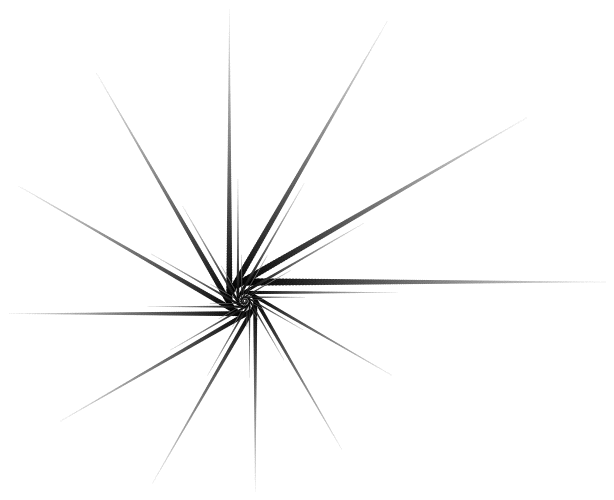
\includegraphics[keepaspectratio,width=\textwidth,height=0.75\textheight]{Nautilus_Star.png}
\label{}
\end{figure}


\end{frame}

\begin{frame}

\frametitle{Another demo}
\label{anotherdemo}

\begin{table}[htbp]
\begin{minipage}{\linewidth}
\setlength{\tymax}{0.5\linewidth}
\centering
\small
\begin{tabular}{@{}lll@{}} \toprule
First&Second&Third\\
\midrule
a longer cell&short&short\\
short&longer cell&short\\

\bottomrule

\end{tabular}
\end{minipage}
\end{table}


\end{frame}

\mode<all>
\input{mmd-beamer-footer}

\end{document}\mode*

